\documentclass[t]{beamer}

\usepackage[english]{babel}
\usepackage[utf8x]{inputenc}
\usepackage{tikz}

\mode<presentation>
{
  \usetheme{Madrid}       % or try default, Darmstadt, Warsaw, ...
  \usecolortheme{default} % or try albatross, beaver, crane, ...
  \usefonttheme{professionalfonts}    % or try default, structurebold, ...
  \setbeamertemplate{navigation symbols}{}
  \setbeamertemplate{caption}[numbered]
  \definecolor{aaublue}{RGB}{33,26,82}% dark blue
  \definecolor{ReneOrange}{RGB}{255,100,0}
  \definecolor{Blaaligfarve}{RGB}{57,51,136}   
  \definecolor{Mindreblaaligfarve}{RGB}{89,78,191}  

  \colorlet{beamer@blendedblue}{aaublue}
} 

\setbeamercolor{date in head/foot}{bg=Mindreblaaligfarve, fg=white}
\setbeamercolor{title in head/foot}{bg=Blaaligfarve, fg=white}
\setbeamercolor{author in head/foot}{bg=aaublue, fg=white}
\setbeamercolor{block title}{bg=Mindreblaaligfarve, fg=white}
\setbeamercolor{block title alerted}{bg=Mindreblaaligfarve, fg=white}
\setbeamercolor{block title example}{bg=ReneOrange, fg=white}

\title[Arduino over 433 MHz]{Arduino peer-to-peer using 433 MHz}
\subtitle{RTS - Presentation}
\author{SW503-E15}
\date{19 OCT 2015}
\begin{document}

\begin{frame}
  \titlepage
\end{frame}

\begin{frame}{Outline}
  \tableofcontents
\end{frame}

\section{Introduction}

\begin{frame}{How to use boxes.}
\begin{blueblock}[An example of the first kind]
  Something about this example of the first kind.
\end{blueblock}
\begin{orangeblock}[An example of the second kind]
  Something about this example of the second kind.
\end{orangeblock}
%\begin{example}[A regular example]
%  Something about the regular example.
%\end{example}
\textcolor{ReneOrange}{text} derp

\end{frame}

\begin{frame}{What is the project about?}
	\begin{block}{What is the project about?}
	 	\begin{itemize}
			\item What are the main problems for the project?
			\item Time Constraints
			\item One channel for communication
			\item Below 100 \% of transmission received
		\end{itemize}
	\end{block}

	\begin{block}{Hardware}
		\begin{itemize}
			\item ATMega microcontroller (Arduino)
			\item 433 MHz Transceivers
			\item Operating System
			\item Intern Schedueling
			\item External Schedueling
		\end{itemize}
	\end{block}

\end{frame}

\begin{frame}{Arduinos}

	\begin{minipage}[0.3\textheight]{\textwidth}
	\begin{columns}[T]
	\begin{column}{0.5\textwidth}
		\begin{figure}
	 	 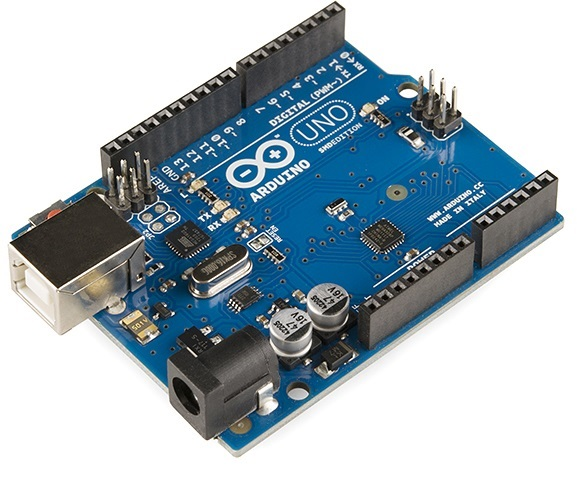
\includegraphics[width=1\textwidth,height=1\textheight,keepaspectratio]{figures/Arduino_Uno.jpg}
	 	 \caption{Arduino Uno}
	 	 \end{figure}
	\end{column}
	\begin{column}{0.5\textwidth}

	 
	 \vspace{2 mm}
	  \begin{figure}
	  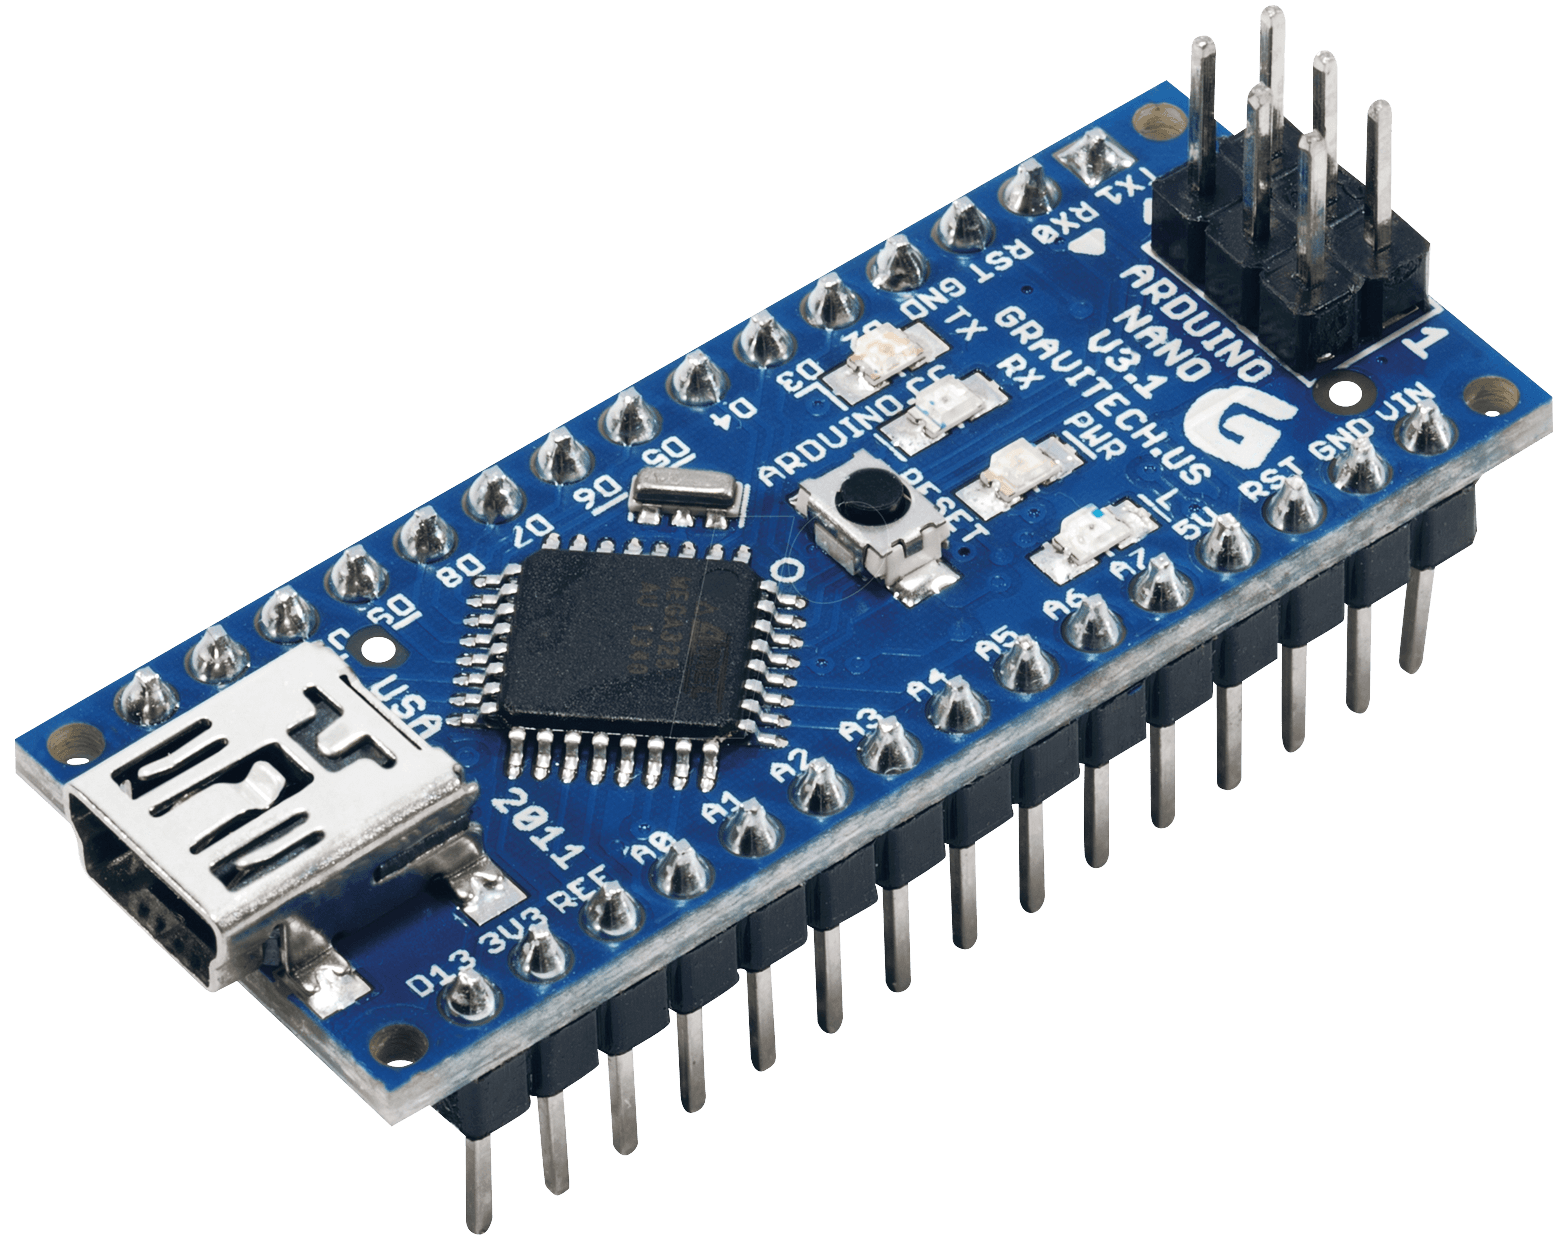
\includegraphics[width=1\textwidth,height=1\textheight,keepaspectratio]{figures/Arduino_Nano.png}
	  \caption{Arduino Nano}
	  \end{figure}
	\end{column}
	\end{columns}
	
  \end{minipage}
\end{frame}

\begin{frame}{What is the project about?}
	\begin{block}{What is the project about?}
	 	\begin{itemize}
			\item What are the main problems for the project?
			\item Time Constraints
			\item One channel for communication
			\item Below 100 \% of transmission received
		\end{itemize}
	\end{block}

	\begin{block}{Hardware}
		\begin{itemize}
			\item ATMega microcontroller (Arduino)
			\item 433 MHz Transceivers
			\item Operating System
			\item Intern Schedueling
			\item External Schedueling
		\end{itemize}
	\end{block}

\end{frame}

\end{document} 